% !TeX program = xelatex
\documentclass{nwputhesis}
\usepackage{gbt7714}
\begin{document}

% 生成封面, 使用\maketitle 
% 该封面不同学院要求可能不同,如有需要,请在cls文件中自行修改
\maketitle

\newpage
% 目录
\makecontent
\iffalse
    \makefigcontent
    \maketabcontent
\fi
% 正文
\maketext

\section{实习目标}
\subsection{学习方向及目标}
学习现在先进的计算机视觉(Computer Vision)以及图形学与AI结合的模型如Neural Radiance Fields(神经辐射场,简称NeRF),3D Gaussian Splatting(3D高斯溅射,简称3dgs),以及YOLO(全称You Only Look Once),同时理解各个模型的实现原理。
\subsection{期望}
\begin{itemize}
    \item 完成搭建尽可能多的AI模型,配置其环境,并完成训练其预设数据库。
    \item 学习并理解各个模型的实现原理。
    \item 自己制作数据并通过基于AI的三维重建制作模型。
\end{itemize}
\makespace
\section{模型的搭建以及学习}
\subsection{Yolo V5}
\subsubsection{模型简介}
Yolo(You Only Look Once)是一种单阶段目标检测算法,即仅需要 “看” 一次就可以识别出图片中物体的class类别和边界框。Yolov5是由Alexey Bochkovskiy等人在YOLO系列算法的基础上进行改进和优化而开发的,使其性能与精度都得到了极大的提升。
\subsubsection{模型环境配置}
\begin{itemize}
    \item Python = 3.8.19
    \item torch = 2.3
    \item torchvision = 0.18.0
    \item gitpython = 2.40.1
    \item opencv-python = 4.9.0.80
    \item matplotlib = 3.7.5
    \item pandas = 2.0.3
\end{itemize}
模型从\underline{https://github.com/ultralytics/yolov5.git}克隆下来,然后在本地进行配置。

\subsubsection{模型训练}
模型训练是在\underline{train.py}文件中进行的,训练时可以同时输入data\footnote{文件中包含了训练集和验证集的路径,以及所有的标注种类}、cfg\footnote{文件中包含了模型的参数,如学习率、batch size等}和weight\footnote{文件中包含了预训练模型的权重}文件;或是epochs\footnote{训练的次数}和batch size\footnote{每次训练的图片数量}。
\\
如下图:
\begin{figure}[H]
    \centering
    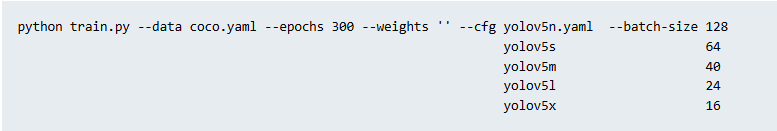
\includegraphics[width=0.8\textwidth]{picture/2.png}
    \caption{YOLOv5目标检测模型的训练命令}
\end{figure}
\subsubsection{测试自己制作的数据集}
从网上找寻了30张宝可梦的图片,然后通过labelImg工具标注这些图片中比较常见的宝可梦,如皮卡丘、杰尼龟等,然后将这些图片和标注文件放入到一个文件夹中。最后通过YOLOv5模型进行训练,得到了一个可以识别这些宝可梦的模型,因为数据集比较小,所以模型的识别率不是很高。
\\
训练结果示例:
\begin{figure}[H]
    \centering
    
\includegraphics[width=0.8\textwidth]{picture/3.png}
    \caption{YOLOv5目标检测模型的训练结果}
\end{figure}
\subsubsection{实现原理}
YOLOv5首先会在输入端中将输入图片进行预处理,图像大小调整为模型所需的大小,进行归一化操作,及将像素值缩放到0到1之间。\\
然后将图片输入到backbone网络\footnote{backbone网络是一个特征提取网络,用于提取图片的特征}中,backbone网络会将图片的特征提取出来,然后将这些特征输入到neck网络\footnote{neck网络是一个特征融合网络,用于将不同层次的特征进行融合}中,neck网络会将不同层次的特征进行融合,然后将这些特征输入到head网络\footnote{head网络是一个预测网络,用于预测图片中的物体}中,head网络会将图片中的物体进行预测,得到物体的类别和边界框。
\\


\makespace
\section{英文标题Test}
\subsection{英文标题Test}
\subsubsection{英文标题Test}
% 参考文献
\makespace
\section*{参考文献}
\begingroup  % 去掉thebibliography环境自带的“参考文献”标题
\renewcommand{\section}[2]{}
\addcontentsline{toc}{section}{参考文献}
% npu专用
\bibliographystyle{gbt7714-numerical}
\addtolength{\itemsep}{-0.6em} % 缩小参考文献间的垂直间距
\begin{spacing}{1.0}           %段落行距设置
    \bibliography{reference/reference}
\end{spacing}
% 参考文献位置

% 致谢
\makespace %另起一页空两行
\section*{致谢}
\begin{center}
    { \blackti \fontsize{16.0600pt}{1.25}致 \, 谢}
\end{center}
\addcontentsline{toc}{section}{致\texorpdfstring{ \, }{} 谢}
\myspace{1}
致谢内容。

% 毕业设计小结
\section*{毕业设计小结}
\makespace
\begin{center}
    { \blackti \fontsize{16.0600pt}{1.25}毕业设计小结}
\end{center}
\addcontentsline{toc}{section}{毕业设计小结}
\myspace{1}
小结内容。

% 附录
\makespace
\section*{附录}
\begin{center}
    { \blackti \fontsize{16.0600pt}{1.25}附 \, 录}
\end{center}
\addcontentsline{toc}{section}{附\texorpdfstring{ \, }{} 录}
\myspace{1}
附录内容。
\end{document}

